\documentclass[tikz,border=8pt]{standalone}
% Shared TikZ style for synorg platform diagrams. Each diagram \input's this
% inside a standalone document. Palette tracks the Material "teal" site theme so
% figures read as one system in light mode (SVGs are theme-neutral otherwise).
\usetikzlibrary{arrows.meta,positioning,shapes.geometric,fit,backgrounds,calc,decorations.pathreplacing}

\definecolor{synteal}{HTML}{00897B}   % primary
\definecolor{synfill}{HTML}{E0F2F1}   % light fill
\definecolor{synamber}{HTML}{B26A00}  % warning / lend
\definecolor{synred}{HTML}{B00020}    % deny / danger
\definecolor{syngrey}{HTML}{5F6368}   % muted

\tikzset{
  >=Stealth,
  font=\sffamily\small,
  box/.style={draw=synteal,line width=0.6pt,rounded corners=2pt,fill=synfill,
              inner sep=5pt,align=center},
  plane/.style={draw=synteal,line width=0.8pt,rounded corners=3pt,fill=synfill,
                inner sep=8pt,align=center},
  state/.style={draw=synteal,line width=0.7pt,circle,fill=synfill,inner sep=3pt,
                minimum size=11mm,align=center,font=\sffamily\footnotesize},
  decision/.style={draw=synteal,line width=0.7pt,diamond,aspect=2,fill=synfill,
                   inner sep=1pt,align=center,font=\sffamily\footnotesize},
  deny/.style={draw=synred,fill=synred!8,text=synred},
  warn/.style={draw=synamber,fill=synamber!10},
  flow/.style={->,line width=0.6pt,draw=syngrey},
  flowlbl/.style={font=\sffamily\footnotesize,text=syngrey,inner sep=2pt},
  note/.style={font=\sffamily\footnotesize\itshape,text=syngrey},
}

\begin{document}
% The four planes (architecture.md "four planes"): a change flows top-to-bottom
% (authored in git, actuated by reconcilers, judged by policy, recorded as
% evidence); evidence flows back up to inform the next change.
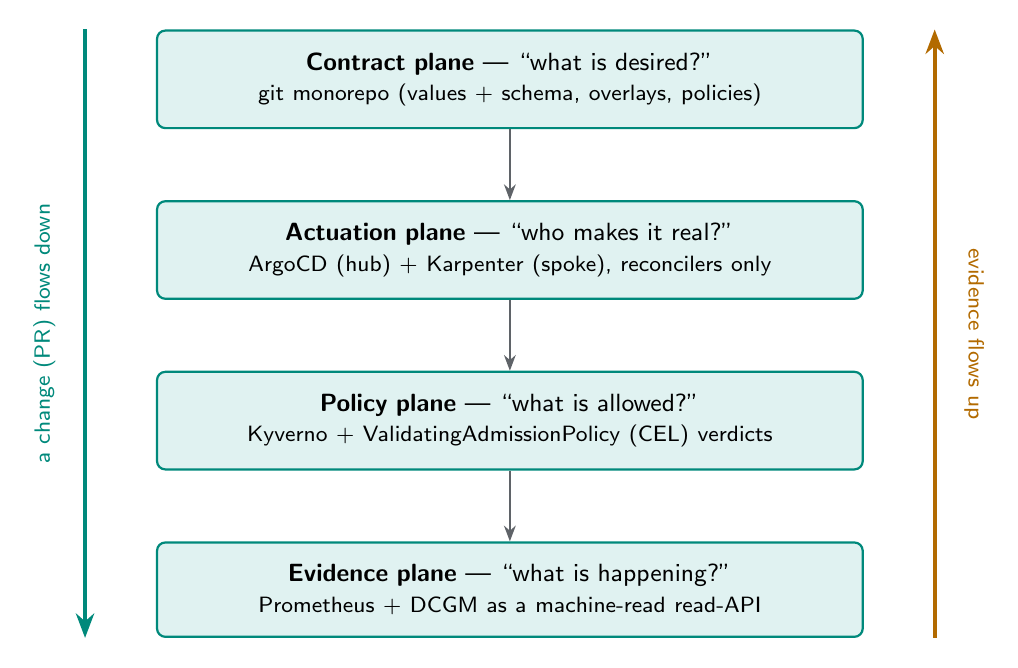
\begin{tikzpicture}
  \def\pw{8.4cm}
  \node[plane,text width=\pw] (contract)
    {\textbf{Contract plane} --- ``what is desired?''\\\footnotesize git monorepo (values + schema, overlays, policies)};
  \node[plane,text width=\pw,below=9mm of contract] (actuation)
    {\textbf{Actuation plane} --- ``who makes it real?''\\\footnotesize ArgoCD (hub) + Karpenter (spoke), reconcilers only};
  \node[plane,text width=\pw,below=9mm of actuation] (policy)
    {\textbf{Policy plane} --- ``what is allowed?''\\\footnotesize Kyverno + ValidatingAdmissionPolicy (CEL) verdicts};
  \node[plane,text width=\pw,below=9mm of policy] (evidence)
    {\textbf{Evidence plane} --- ``what is happening?''\\\footnotesize Prometheus + DCGM as a machine-read read-API};

  % inter-plane hand-off
  \draw[flow] (contract) -- (actuation);
  \draw[flow] (actuation) -- (policy);
  \draw[flow] (policy) -- (evidence);

  % a change flows down (left rail)
  \coordinate (tl) at ($(contract.north west)+(-0.9,0)$);
  \coordinate (bl) at ($(evidence.south west)+(-0.9,0)$);
  \draw[flow,line width=1.3pt,draw=synteal] (tl) -- (bl);
  \node[flowlbl,text=synteal,rotate=90,anchor=south] at ($(tl)!0.5!(bl)+(-0.3,0)$)
    {a change (PR) flows down};

  % evidence flows back up (right rail)
  \coordinate (br) at ($(evidence.south east)+(0.9,0)$);
  \coordinate (tr) at ($(contract.north east)+(0.9,0)$);
  \draw[flow,line width=1.3pt,draw=synamber] (br) -- (tr);
  \node[flowlbl,text=synamber,rotate=-90,anchor=south] at ($(br)!0.5!(tr)+(0.3,0)$)
    {evidence flows up};
\end{tikzpicture}
\end{document}
